\cotefile{161-3}
\scanpage{41}
(We can take for $C$ any subcategory of $E$ which \deleted{is} generates \uline{$E$}, in the sense we've explained, and take $E\xrightarrow{f_*}\widehat C$ by \uline{$f_*(X)=(A\mapsto\operatorname{Hom}(A,X))$} \deleted{(associating to each)}. To say that this functor is conservative means that \deleted{the} $C$ \deleted{\unsure{is}} generating, and this \deleted{does imply that} is equivalent with $f_*$ fully faithful, and implies the existence of the left adjoint $f^*$ ....)

% slanted
\margin{\unsure{Epimorphic} families are strict, and \unsure{there are|then are|their} kernels and \deleted{the} fibered products (\deleted{conserv.} \deleted{$f_*$ \unsure{is}} \unsure{Cons.} functor $\Rightarrow$ \unsure{can.} $\Rightarrow$ $\varphi$ \unsure{faithful} $\Rightarrow$ $\varphi$ fully faithful}

\uline{Generators} Useful in various contexts: existence of equalizers \inserted{(obvious, or otherwise)}, \deleted{or proving that any functor from} hence together with generators, existence of \uline{cogenerators}, and \margin{\uline{technical}} the fact that \deleted{functors} \inserted{cov(contravar)} to Sets (say) that transforms $\varprojlim$ ( $\varinjlim$ into $\varprojlim$ are representable.

\uline{NB} Recall that a topos has \unsure{``cohomology|``category|``cohomotopy} and homotopy invariants $\left\{\begin{array}{ll}\operatorname{Top}(\varnothing)&\text{\uline{empty topos}}\\ \operatorname{Top}(\mathbf1)&\deleted{\unsure{one}}\ \text{\uline{point} (or final) topos.}\end{array}\right.$

% slanted
\margin{we will \unsure{admit|grant} that \unsure{equivalent} categories define ``essentially same'' topos}

\deleted{\illegible{1}} \uline{Examples} a) $\operatorname{Top}(X)$. \inserted{\unsure{of} two systems of \unsure{gen} $C\in E$ ..}

\[\operatorname{Top}(X,G),\qquad\left\{\begin{aligned}\operatorname{Top}(X,e)&=\operatorname{Top}(X)\\\operatorname{Top}(\unsure{e|1|*},G)&=\deleted{\unsure{B}}B_G.\quad H^i(B_G,\ )=H^i(G,\ )\end{aligned}\right.\]

% slanted
\margin{\unsure{Cohomologie} mixte \deleted{\unsure{de}} en $X,C$ Cohomologie \unsure{de|en} $G$}

Here fiber functor \inserted{of $B_G$} is \uline{forget}ful functor, it has automorphisms.! \inserted{We get more generally as fiber-functors for $B(X,G)$, \unsure{automorphisms} from \unsure{the} stabilizer \unsure{Gp} \unsure{of} $x$ ...}

$\underline{\mathrm{b})}\quad\widehat C$ (from algebra) -- generalizes $B_G$.

\[C^\circ\longrightarrow\underline{\mathrm{Fib}}(\widehat C)^{\deleted{\unsure{e}}}\qquad\text{(we can prove this induces}\] \[\text{\uline{fully faithful}}\qquad\operatorname{Ind}(C^\circ)\simeq\underline{\mathrm{Fib}}(\widehat C)\ .\]

% slanted
\margin{Cohomologie de $C$ liens \unsure{(x)} ...! $\leftarrow$ topos d'homotopie fort généraux}

\uline{Question} Can we have an equivalence $\widehat C\simeq\operatorname{Top}(X)$ (look at fiber functors), \deleted{this implies} \inserted{yes we \unsure{see} and suffices that} $C$ is an \uline{ordered category}, \deleted{\unsure{and}} and \deleted{that $X$ has \deleted{\unsure{extre}} enough pts which have a smallest neighbourhood (``essential points'') -- they would be everywhere dense -- $C$ could be interpreted as contained in the set of those pts of $X$, with the induced order relation} we can then take $X$ as $\operatorname{Ind}(C)$ (add to $C$ $\operatorname{Inf}$ of decreasing families) and \unsure{endow} with topology ....
% archive sheet number: 40
\scanpage{42}
% sheet rotated 180 degrees; diagonal cancellation across the draft
\deleted{pas néc. celle des corps). La question a une solution affirmative ssi tout \deleted{anneau} $C\in\operatorname{ob}(\mathrm{Ann})$ tel que, pour tout $(u:A\to B)\in M$, $\operatorname{Hom}(B,C)\xrightarrow{\sim}\operatorname{Hom}(A,C)$ bij, $C$ est un \uline{corps}.}

\deleted{Prenons donc d'abord $\lambda=\unsure{\varnothing_{\lambda_0}|\lambda_0|\mathcal E\lambda_0}$, donc les objets des $S^T_\lambda$ \inserted{resp} $(R^T_\lambda)$ sont les anneaux de polynômes sur $\mathbb Z$ \inserted{(à un nb fini de variables)}}

\deleted{[top. des \deleted{\unsure{espaces|équations}} \inserted{schémas isomorphes aux schémas} affines types de type fini $\mathbb E^{\unsure{n|\mathbb Z}}_{\mathbb Z}$ sur $\mathbb Z$]}

\deleted{Si $u:\underset{\underset{\mathbb E^m}{\unsure{\simeq|\lambda}}}{X}\longrightarrow\underset{\mathbb E^n}{Y}$ est dans $M\deleted{\unsure{e|\mathcal C}}$, on sait que $m=n$, et \deleted{que} que c'est un isom fibre par fibre (Main theorem de Zariski) donc que c'est un isom. \deleted{(Grauert via Zariski} Donc $M'$ est réduit aux isomorphismes, donc $M$ aussi, on aurait donc que $(\mathrm{Ann})^*=\mathrm{Ann}$, absurde !}

\deleted{b) Supposons \deleted{\unsure{plutôt}} que $\lambda=(\underset{\leftarrow}{\lambda},\underline{\lambda}=\varnothing)$, et que $S^T_\lambda$ contient, en plus \deleted{\unsure{des}} de $\mathbb Z[t]$, les anneaux $\mathbb Z[t,t^{-1}]$ (ce qui est vrai si $\underset{\leftarrow}{\lambda}=$ ens des tous les diagrammes finis -- auquel cas $S^T_\lambda=$ ens. des anneaux de type fini sur $\mathbb Z$). Alors la flèche canonique}

\[\deleted{u_0:\mathbb Z[t]\longrightarrow\mathbb Z[t,t^{-1}]\times\mathbb Z\quad\bigl(\simeq\mathbb Z[x,y]/\bigl(\deleted{\unsure{xy,xy-1}}\,\inserted{x(xy-1),y(xy-1)}\bigr)\bigr)}\]

\deleted{qui applique $t$ dans $(t,0)$, \inserted{[ou $x$ dans $\dot x$]} est dans $M$, et plus précisément, pour tt anneau $C$, le transformé par $u_0$ par $\operatorname{Hom}(-,C)$ est l'application \inserted{(injective)} qui, à toute \deleted{couple} décomposition \deleted{$\unsure{(x,y)}\quad C^*\times\{\unsure{0|e}\}\to C$} de $C$ en $C_1\times C_2$ (i.e. de $\unsure{Z|X|\mathcal X}=\operatorname{Spec}C$ en $Z\simeq Z_1\amalg Z_2$) et à tout élément \deleted{qui associe à $C$} inversible \inserted{$f$} de $C_1^{\deleted{\unsure{*|\#}}}$, associe l'élément $(\unsure{f|g|\varepsilon},0)$ de $C$.}

\deleted{Cette application est bijective ssi $C$ est un corps [prouvons d'abord que $X=\operatorname{Spec}C$ est connexe i.e. $C$ n'est pas isom. à un produit $C_1\times C_2$ avec $C_1,C_2\ne0$}
% archive sheet number: 41
\scanpage{43}
c) Soit $G$ un groupe d'un Topos, \uline{Topos classifiant} $B_G$. (Il ``classifie'' les torseurs sous $G$ -- mais

\margin{\deleted{\unsure{Topos} \unsure{étalé}}}

\deleted{\unsure{$B_G$}} d) \uline{Topos induit} $E_{/X}$ (on identifie \unsure{souvent} $E$ avec son objet final, $E_{/X}$ avec $X$ ... )

\margin{\uline{l'objet} \uline{hom} \uline{\unsure{endomorphismes|homomorphismes}} \unsure{de} catégorie \uline{triviale}}

3) Morphismes de topos : \uline{forment une catégorie.}

\[\begin{aligned}\underline{\mathrm{MorTop}}(X,Y)&\lhook\joinrel\xrightarrow[\mathrm{plfid}]{}\underline{\mathrm{Hom}}\ \underline{\mathrm{cat}}\,(X,Y)\\ f&\longmapsto f_*\end{aligned}\]

% slanted
\margin{$\bullet$ Attention sens des flèches}

La composition des morphismes est un \unsure{accouplement} \deleted{Morphisme} de catégories, i.e. associatif : les topos forment une ``2-catégorie'' (pas seulement une catégorie).

% slanted
\margin{Attention ne pas passer trop hâtivement aux classes d'isomorphie des topos.}

Notion d'équivalence \inserted{de topos} : $f:X\to Y$ est une équivalence ssi $\exists\,g:Y\to X$ t. q. $gf\simeq\mathrm{id}_{\deleted{\unsure{Y}}X}$, $fg\simeq\mathrm{id}_Y$. Ici, c'est la notion habituelle d'équivalence de catégorie. C'est la notion qui remplace la notion d'isomorphie (= homéomorphie) pour les espaces topologiques.

4) Exemples de morphismes de topos

a) Cas de $\operatorname{Top}(X)$ : déjà étudié : $\operatorname{Top}(X)$ dépend de $X$ de façon covariante. On les identifie. $(\mathrm{Esp\ sob})$ \deleted{\unsure{$\to$}} peut être transformé en 2-catégorie. On a un foncteur 2-fidèle de cette \unsure{dernière} dans la 2-catégorie $(\mathrm{Top})$

a') (Cas de $\operatorname{Top}(X,G)$. \inserted{$(X,G)$ variable} (il n'y a plus de pleine fidélité

b) [Morphismes de $E$ dans $\operatorname{Top}(X)$ : pareil que \deleted{\unsure{foncteur|foutes}} applications $\operatorname{Ouv}(X)\longrightarrow\underbrace{\text{Ss-objets de }e_E}_{\text{ouverts de }E}$, commutant aux sup quelc. et aux $\cap$ finies.]

\uline{Ex} Si $X$ est un \uline{doublet} \inserted{(on écrit $\underline D$)}

\figure{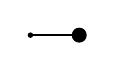
\begin{tikzpicture}[baseline=-.5ex]\draw[line width=.7pt] (0,0)--(.62,0);\fill (0,0) circle (.035);\fill (.62,0) circle (.095);\end{tikzpicture}}

($X=\{x,y\}$, \deleted{\unsure{$x\ne y$}} \deleted{$x\in\overline{\{y\}}$, $y\notin\{x\}$ $\{x\}$} $x$ fermé, $x\ne y$, $x\in\overline{\{y\}}$), alors la donnée de $E$ dans $\operatorname{Top}(X)$ équivaut à la donnée d'un ouvert de $E$ (\deleted{le Topos} \inserted{\unsure{l'objet|des} doublet} est topos classifiant pour l'espèce de structure : ss-objet de l'objet final)

\uline{NB} Tout espace top. de préordre se plonge dans un produit de doublets $\underline D^{I}$
% archive sheet number: 42
\scanpage{44}
% sheet rotated 180 degrees
\diagram{\begin{tikzcd}[ampersand replacement=\&,column sep=small,row sep=small] \& S'\arrow[dr]\&\\ \unsure{\mathscr S|S}\arrow[ur]\arrow[rr,-]\&\& R\end{tikzcd}}

\[\underline{\mathrm{Hom}}_\lambda(R,Z)\xrightarrow[\mathrm{fid}]{}\underline{\mathrm{Hom}}_\lambda(S',Z)\lhook\joinrel\xrightarrow[\mathrm{pl.fid}]{}\underline{\mathrm{Hom}}_\lambda(S,Z)\]

\[\lambda\subset\lambda'\qquad (\mathrm{Cat}_{\lambda'})\longrightarrow(\mathrm{Cat}_{\lambda})\]

\margin{$T(\mathrm{Ens})$ $R_T^\lambda$ en fonction de $T(\mathrm{Ens})$ ?}

% diagonal stroke runs from below the inclusion through these rows into the lower working
\diagram{\begin{tikzcd}[ampersand replacement=\&,column sep=large] \unsure{\mathrm{Cat}/\mathrm{cofib}|\mathrm{Cat}\supset\mathrm{cofib}}(\mathrm{Cat}_{\lambda})\arrow[r,Rightarrow]\&\unsure{\mathrm{Cat}/\mathrm{cofib}|\mathrm{Cat}\supset\mathrm{cofib}}(\mathrm{Cat}_{\lambda'})\\ (\unsure{\lambda:\mathrm{types}|\lambda\text{-types}})\arrow[u,hook]\arrow[d,hook]\arrow[r,dashed,"{?}"]\&(\lambda'\text{-types})\arrow[u,hook]\arrow[d,hook]\\(\mathrm{Cat}_{\lambda})\arrow[r,shift left,"{\deleted{\longrightarrow}}"]\arrow[r,dashed,shift right]\&(\mathrm{Cat}_{\lambda'})\end{tikzcd}}

\deleted{$\left\{\begin{array}{l}\lambda'\text{-catégorie}\\\text{enveloppante}\\\text{d'une }\lambda\text{-catégorie}\end{array}\right.$}

\diagram{\begin{tikzcd}[ampersand replacement=\&] C\arrow[r,hook]\arrow[d,Rightarrow]\&(\check C)^\circ\\ X\unsure{.|{}_{i}}\&\end{tikzcd}}

\[\deleted{\underline{\mathrm{Hom}}(R,C^\circ)^\circ\simeq\underline{\mathrm{Hom}}(R^\circ,C)^{\deleted{\unsure{\circ}}}}\]

\diagram{\begin{tikzcd}[ampersand replacement=\&] C\arrow[r,hook,"{\lambda\text{-fonct}\deleted{\unsure{r}}}"',"{\text{\uline{pl. fid}}}" description]\& C'\arrow[dr]\\ \&\&{}\end{tikzcd}}

\diagram{\(\left\{\vcenter{\hbox{\begin{tikzcd}[ampersand replacement=\&,column sep=small] \deleted{\unsure{R}}\quad T(C)\& C^{\circ I}\&\\ \underline{\mathrm{Hom}}_\lambda(R,C)\arrow[r,hook,"{\unsure{\mathrm{2\text{-}cat}|\mathrm{2\text{-}cart}}}"']\arrow[d,hook]\&\underline{\mathrm{Hom}}_\lambda(R,\widehat C)\arrow[d,hook]\& C\arrow[r]\& C^I\\ \underline{\mathrm{Hom}}_{\deleted{\unsure{\mathrm{cat}}}}(R,C)\arrow[r,hook]\arrow[d,"{\varphi_C}"']\& \underline{\mathrm{Hom}}_{\unsure{\lambda}}(R,\widehat C^{\deleted{\unsure{I}}})\arrow[d,"{\varphi_{\widehat C}}"]\\ C^I\arrow[r,hook]\&\widehat C^{I}\end{tikzcd}}}\right.\)}

\diagram{\begin{tikzcd}[ampersand replacement=\&] \deleted{\unsure{\mathrm{Ex}}}\ T_\lambda(C)\arrow[d]\&T_\lambda(C')\arrow[l,hook]\arrow[d]\\ C^{\unsure{I|+}}\& {C'}^I\arrow[l,hook]\end{tikzcd}}

\diagram{\begin{tikzcd}[ampersand replacement=\&,column sep=small] T(\mathrm{Ens})\arrow[r,equal]\&\underline{\mathrm{Hom}}_\lambda(R,(\mathrm{Ens}))\\ R_T\arrow[r,Rightarrow]\&\underline{\mathrm{Hom}}(T(\mathrm{Ens}),\mathrm{Ens})\arrow[d]\\R_T\arrow[r,shift left,"\simeq"]\&\underline{\mathrm{Hom}}(T(\mathrm{Ens})_{\varnothing},(\mathrm{Ens}))\arrow[l,shift left,"{\unsure{\text{plus gén.}|\text{quelque}}}"']\end{tikzcd}}

1) \unsure{Réduction|Résolution|Rigidité} : $\widehat C$ \qquad 2) Existence des $\varprojlim$ \deleted{\unsure{quelc.}} de type $\lambda$ dans \inserted{les} $T(C)$ (commutation avec $\underset{\leftarrow}{\lambda}$ et $\underline\lambda$)
% separate long bracket to the left of the list
3) Existence des $\varinjlim$ dans les $T(C)$ si ... \unsure{??|(?)} \quad 4) Adjoint de $\varphi:T(\mathrm{Ens})\to(\mathrm{Ens})^I$ dans $T(\mathrm{Ens})$ si $\lambda$ est \deleted{\unsure{fini|formé}} de diag \uline{finis} \quad 5) $R_T\simeq\underline{\mathrm{Hom}}(T(\mathrm{Ens})_\circ,(\mathrm{Ens}))$ ?? \inserted{objets de t. f.}
% archive sheet number: 43
\scanpage{45}
(\unsure{ici|i.e.} on peut prendre $\unsure{I|J}=\operatorname{Ouv}(X)$).

\deleted{\unsure{a)}} \uline{NB} Si l'ens. des ouverts de $E$ est \deleted{\unsure{un}} isomorphe (pour la structure ordonnée) à l'ens des ouverts $\operatorname{Ouv}(X)$ quelque $X$, alors $E\to\deleted{\unsure{X}}$ \inserted{(i.e. $E\to\operatorname{Top}(X)$)} \unsure{est|c'est|et} \unsure{l'un|un|c'est} universel pour les morphismes de $E$ dans un espace topologique.

\deleted{c) $\operatorname{Top}(X,G)$ pour \unsure{$(X,G)$ variable} les Morphismes de \inserted{$E\xrightarrow[\substack{\varinjlim\\\varprojlim\ \mathrm{fin.}}]{}\underline{\mathrm{Hom}}(\unsure{\mathrm{Cl}^\circ|C^\circ|\mathcal A(X)},\mathrm{Ens})\Longleftrightarrow\unsure{\mathrm{Cl}^\circ|C^\circ}\to\underline{\mathrm{Hom}}(E,(\mathrm{Ens}))$} \unsure{$\underline{\mathrm{Hom}}(\mathrm{Pt}(E))\Leftrightarrow U^\circ\to\underline{\mathrm{Hom}}(\mathrm{Cl},(\mathrm{Ens}))$}}

c) Morphismes d'un pt dans Topos $E$ : Catégories $\underline{\mathrm{Pt}}(E)\simeq\underline{\mathrm{Fib}}(E)^\circ$

d) \uline{Catégories} $\widehat C$ : Tout \deleted{morphisme} \inserted{foncteur} $u:C\to\unsure{C'|\widehat C'}$ définit un foncteur \unsure{?} en sens inverse \inserted{$u^*_{\deleted{\unsure{*}}}\deleted{\unsure{(F)}}:$} $F'\mapsto F'\circ u$

\[\widehat C'\xrightarrow{u^*}\widehat C\]

\deleted{qui a deux adjoints, notés $u_{\unsure{?|!}}^{\deleted{\unsure{*}}}$ et $u^!$} qui commute \deleted{$u^!\ \unsure{u_*u^*}$} \inserted{$u^*\ u_*\ u_!$} aux $\varprojlim$ quelc. et \deleted{le foncteur $u^*$} $\varinjlim$ quelc., donc est le foncteur image inverse pour un $u:\widehat C\longrightarrow\widehat C'$. \inserted{$u_!\quad u^*\quad u_*$}

% slanted
\margin{donc $\widehat C$ est \uline{covariant} en $C$}

En plus de l'adjoint à droite $u_*$, il a un adjoint à g, qu'on note $u_!$ ....

\uline{Ex} : $B_G$ avec $G$ variable, qui est aussi exemple de 4.1. a)

\unsure{$\leftarrow$|e)} [ Morphismes \inserted{de topos} $\widehat C\longrightarrow\unsure{E|\widehat E}$

\[E\xrightarrow[\substack{\varinjlim\\\varprojlim\ \mathrm{finie}}]{}\underline{\mathrm{Hom}}(C^\circ,\mathrm{Ens})\quad\Longleftrightarrow\quad C^\circ\longrightarrow\underbrace{\underline{\mathrm{Hom}}_{\substack{\varinjlim\\\varprojlim\ \mathrm{finie}}}(E,(\mathrm{Ens}))}_{\parallel\,\underline{\mathrm{Pt}}(E)^\circ}\]

\[\underline{\mathrm{Hom\,top}}(\widehat C,E)\simeq\deleted{\unsure{\underline{\mathrm{Hom}}(C^\circ,\underline{\mathrm{Pt}}(E)^\circ)^\circ|\underline{\mathrm{Hom}}(C^\circ,\underline{\mathrm{Pt}}(E)^\circ)}}\ \underline{\mathrm{Hom}}(C,\underline{\mathrm{Pt}}(E))\]

si $E=\widehat C'$, on trouve $\underline{\mathrm{Hom\,top}}(\widehat C,\widehat C')\simeq\underline{\mathrm{Hom}}(C,\deleted{Pt}\operatorname{Pro}\,C')$ \inserted{$(\underline{\mathrm{Hom}}(C,C')\ \mathrm{pl.fid})$}

[ Si $C$ stable par $\varprojlim$ finies, on trouve

\[\underline{\mathrm{Hom\,top}}(E,\widehat C)\simeq\underline{\mathrm{Hom}}_{\mathrm{ex.g.}}(C,E)^\circ\ \Bigr]\vphantom{\widehat C}\]
% archive sheet number: 44
\scanpage{46}
% sheet rotated 180 degrees
$\lambda=(\underset{\leftarrow}{\lambda},\varnothing)$ \qquad muni du foncteur de cat. 2-cofibrées $T\xrightarrow{b^T_{\unsure{\tau|?|C}}}\tau^I$

1) $T$ catégorie \unsure{2-cofibrée|1-cofibrée|$\lambda$-abstraite} sur $(\mathrm{Cat}_\lambda)$. On suppose que \deleted{pour \unsure{tte} $C$}

a) Pour tt foncteur pl. fidèle, $i:C\to C'$ dans $\mathrm{Cat}_\lambda$, $T(i):T(C)\to T(C')$ pl. fid.

\deleted{b)} et le carré

\diagram{\begin{tikzcd}[ampersand replacement=\&] T(C)\arrow[r]\arrow[d,"{b^T_C}"']\&T(C')\arrow[d,"{b^T_{C'}}"]\\ C^I\arrow[r]\&{C'}^I\end{tikzcd}}

est 2-cartésien [il \unsure{le} suffit pour $C\lhook\joinrel\xrightarrow{i'}\widehat C$]

% slanted
\margin{Attention au cas où $\widehat C$ n'est pas une $\mathcal U$-catégorie !}

b) Pour tt $C\in\mathrm{Ob}\,\mathrm{Cat}_\lambda$, le foncteur canonique

\[T(\widehat C)\longrightarrow\underline{\mathrm{Hom}}(C^\circ,\mathscr S)\qquad \mathscr S\overset{\mathrm{déf}}=T(\mathrm{Ens})\]

est une équivalence de catégories.

Alors $T\deleted{\unsure{(C)}}$ se réconstitue à partir de la donnée de $\mathscr S$ et de $(\beta=b_{\mathrm{Ens}}):\mathscr S\to(\mathrm{Ens})^I$, $(\beta=(\beta_i)_{i\in I},\ \beta_i:\mathscr S\to(\mathrm{Ens}))$ comme $T(C)=$ ss-catégorie pleine de $\underline{\mathrm{Hom}}(C^\circ,\mathscr S)$ formée des $\varphi:C^\circ\to\mathscr S$ tels que $\forall i\in I$, $\beta_i\circ\varphi$ soit représentable.

\margin{Mais si $f:C\to C'$ est un $\lambda$-foncteur, comment définir $T(f):T(C)\to T(C')$ en termes de $\mathscr S$, $(\beta_i)$ ?}

\deleted{\unsure{Il suffit}} La ss-catégorie pleine $R$ de $\underline{\mathrm{Hom}}(\mathscr S,(\mathrm{Ens}))$ formée des foncteurs $\psi\deleted{\unsure{g}}$ tels que pour tt $C\in\mathrm{Ob}\,\mathrm{Cat}_\lambda$ \deleted{\unsure{$\xi$}} et $\xi\in T(C)$, le composé $\psi\circ\xi:C^\circ\longrightarrow\mathscr S\xrightarrow{\psi}(\mathrm{Ens})$ soit représentable, est stable par $\varprojlim$ de type $\in\underset{\leftarrow}{\lambda}$, \deleted{A quelle condition} et pour tout $C\in\mathrm{Ob}\,\mathrm{Cat}_\lambda$, on a un accouplement

\[T(C)\times R\longrightarrow C\qquad\substack{\text{commutant aux }\varprojlim\text{ de}\\\text{type }\underset{\leftarrow}{\lambda}\text{ sur }R}\]

d'où $T(C)\to\operatorname{Hom}_{\lambda}(R,C)$ (fonct. de cat. 2-cof. sur $\mathrm{Cat}_\lambda$)

À quelle condition cela est-il une équivalence de catégories ?

Il est néc que a) $R$ soit \inserted{formée de fonct.} repr. i.e. $R\simeq\Sigma^\circ$, où $\Sigma$ est une sous-catégorie pleine de $\mathscr S$ [dans laquelle les $\varinjlim$ (\unsure{inductives|coinductives|inductibles}) de type $\lambda$ existent dans $\mathscr S$, et appartiennent à $\Sigma$]. Donc la donnée de $R$ équivaut à la donnée de $\Sigma\subset\mathscr S$

b) $\Sigma$ engendre $\mathscr S$ $[\,\mathscr S\to\underline{\mathrm{Hom}}(\Sigma^\circ,(\mathrm{Ens}))=\widehat\Sigma\ \text{pl. fidèle}\,]$
% archive sheet number: 45
\scanpage{47}
e) \uline{Morphismes dans topos final} \inserted{$\operatorname{Top}(1)$} Objets constants, foncteur sections.

f) Morphisme du topos vide dans un topos. Morphisme dans le topos vide $E\longrightarrow\deleted{\unsure{E|\mathrm{Ens}}}\operatorname{Top}(\varnothing)$ \deleted{\illegible{1}} : existe ssi $E\simeq\operatorname{Top}(\varnothing)$ i.e. $E$ équivalent à cat. ponctuelle (ou encore tous les objets isom, ou encore l'unique morphisme $\varnothing_E\to e_E$ un isom ....)

g) Classifying $B_G$ ($G$ group of a topos) for variable group object $G$. $E\rightleftarrows B_G$ correspond à $e\rightleftarrows G$

h) Morphisme $E_{/X}\longrightarrow E$ \uline{d'induction}

% slanted
\margin{morphismes $E'\to E$ qui \unsure{sont|$2^\circ$} des \unsure{isom} locaux (ou \uline{\unsure{étalements}} ....)}

\margin{foncteur de localis\deleted{\unsure{tis}}ation, morphisme de localisation}

\[\left\{\begin{aligned}u^*(Y)&=Y_X\\u_!(Y)&=Y\quad(\text{oubli flèche \unsure{structural|structurale|structure}})\\u_*(Y)&\quad\text{plus \unsure{canulé|caché|compliqué}}\end{aligned}\right.\]

Ici \deleted{\unsure{$u$}} $u_!\ u^*\ u_*$, $u^*$ commute aux $\varprojlim$ quelconques .---

$E_{/X}$ \deleted{\unsure{--}} comme foncteur en $X$ -- On peut dire $\underline{\mathrm{Hom\,top}}_E(E_{/X},E_{/Y})\simeq\text{Catégorie discrète de ``set'' }\operatorname{Hom}(X,Y)$

i) \uline{Topos somme} de \uline{topos}
% archive sheet number: 46
\scanpage{48}
Donc $\beta$ \inserted{$(\beta_i)$} s'interprète en termes de cat. des \unsure{constructions|construct.} (resp. constr. \unsure{infinies|inférieures})

$\lambda$ ens de types de diagrammes \uline{finis}

% long diagonal cancellation from line 4 to the last line
\diagram{\(\left\{\vcenter{\hbox{\begin{tikzcd}[ampersand replacement=\&,row sep=small,column sep=small] \deleted{\Sigma}\&\deleted{\text{catégorie stable par }\varinjlim\text{ de type }\lambda}\\ \deleted{R}\&\deleted{{}=\Sigma^\circ}\\ \deleted{\mathscr S}\&\deleted{{}=\underline{\mathrm{Hom}}_\lambda(R,\mathrm{Ens})\deleted{\unsure{\subset|\mathrm{Ens}}}\,\widehat\Sigma}\\ \deleted{\Sigma}\arrow[u,hook]\&\end{tikzcd}}}\right.\)}

\deleted{Je dis que a) $\mathscr S$ admet des $\varinjlim$ quelc.}

\deleted{b) Pour tte catégorie \inserted{$\mathscr T$} ayant des $\varinjlim$ quelc, On a}

\diagram{\begin{tikzcd}[ampersand replacement=\&,row sep=small] \&\deleted{\underline{\mathrm{Hom}}_{\underset{\rightarrow}{\lambda}}(\Sigma,\mathscr T)}\&\deleted{\underline{\mathrm{Hom}}_{\underset{\rightarrow}{\lambda'}}(\mathscr S,\mathscr T)}\arrow[l,"\simeq"']\arrow[l,shift left,shorten >=2pt,shorten <=2pt,<-]\\\deleted{\underline{\mathrm{Hom}}_{\underset{\leftarrow}{\lambda}}(R,\mathscr T^\circ)}\arrow[ur,equal]\arrow[d,equal]\&\&\\\deleted{T(\mathscr T^\circ)}\arrow[rr,bend right]\&\&\deleted{\underline{\mathrm{Hom}}_{\underset{\leftarrow}{\lambda'}}(\mathscr S^\circ,\mathscr T)}\arrow[ll,"\simeq"']\end{tikzcd}}

\deleted{où $\underline{\mathrm{Hom}}_{\lambda'}$ désigne les foncteurs commutant aux $\varinjlim$ quelconques.}

\deleted{$\mathscr S$ est engendré par $\varinjlim$ par $\Sigma$}
% archive sheet number: 47
\scanpage{49}
Comparison between topoi $\widehat C$ and $\unsure{\operatorname{Topol}|\operatorname{Top}}(X)$

$\widehat C$ is $\simeq$ to a $\operatorname{Top}(X)$ iff $C$ is an ordered category (i.e. $\forall x\in\mathrm{ob}\,C$, $x\to e_{\widehat C}$ is a monomorphism)

When this is so, we can take $X$ to be $C$ with the topology generated by the sets $O_x=\{y\in C\mid y\leq x\}$ i.e. arbitrary unions [of intersections] of such sets : in fact \deleted{[NB $x\in\overline{\{y\}}$ iff $y\leq x$] i.e. $y\in O_x$] \unsure{of} Open} the $O_{\unsure{i|x}}$'s form a \uline{basis} of the topology, and open \deleted{On the other hand, if $X$ is an} sets \inserted{$O$} are \deleted{those which} the \deleted{crible's} sieve's

\[\bigl(\deleted{\forall x\in O,\ \unsure{\Longrightarrow|\Longleftrightarrow}}\ (y\leq x\text{ and }x\in O\Longrightarrow y\in O)\ .\ \deleted{\text{and }O=\bigcup_xO_x\ldots}\]

\deleted{If $F$ is a Functor on $C$, then $F(O)\longrightarrow\prod F(O_{x_{\unsure{i|j}}})\rightrightarrows\prod F$}

Thus sheaves on $C$ are just the sheaves on this basis of open sets, i.e. contravariant functors $O_x\to F(O_x)=F(x)$ from $C'$ \deleted{\unsure{$C$} to \unsure{$\xi$} sets} (category of all $O_x$, $O_y\hookrightarrow O_x$ iff $y\leq x$) $\simeq C$ to sets, satisfying the sheaf property \deleted{with} with respect to \deleted{cover \unsure{sieves} of} \inserted{coverings} of $O$ ; but these are trivial (for if $O_{x_i}$ cover $O_x$, $\exists\,i$ s.th $x\in O_{x_i}$ i.e. $\deleted{x_i}x\leq x_i$ hence $x\simeq x_i$ (as $x_i\leq x$) then we'll get arbitrary presheaves

Conversely, if $X$ is a sober space, then $\operatorname{Top}(X)$ is $\simeq$ \inserted{to an} $\widehat C$ iff the \deleted{\unsure{closed}} \inserted{essential} points of $X$ (i.e. those which have a smallest open neighbourhood -- or those for which the fiber functor commutes with products) are very dense [and we may take for $C$ the category of those pts).
% archive sheet number: 48
\scanpage{50}
\diagram{\begin{tikzcd}[ampersand replacement=\&] B_G\arrow[d]\& (Z,G)\\ B_e\&\end{tikzcd}}

% block below is rotated 180 degrees relative to the group above
\margin{Prasad Gopal}

\diagram{\begin{tikzcd}[ampersand replacement=\&,column sep=large] \deleted{C}\arrow[r,"f"]\arrow[r,dashed,shift right=1.3ex,<-,"g"']\arrow[r,dashed,shift right=2.6ex,"{\deleted{\unsure{g}}\,h}"']\&\deleted{C'}\\ {}\arrow[r,-]\&{}\\ \deleted{\widehat C}\arrow[r,shift left=1.6ex,"{f_!}"]\arrow[r,shift right=1.6ex,"{f_*}"']\&\deleted{\widehat C'}\arrow[l,"{f^*}"']\end{tikzcd}}

\deleted{$\widehat f:\widehat C\to\widehat C'$ morphisme de topos $\left\{\begin{aligned}\widehat f^*&=f^*\\\widehat f_*&=f_*\end{aligned}\right.$ \quad $\widehat f_!=f_!$}

\deleted{$f_!$ prolonge $f$ \quad $f^*$ prolonge $g$ (si $g$ existe) \quad $f_*$ prolonge $h$ (si $h$ existe)}

\[\begin{aligned}&\deleted{\operatorname{Hom}_{\widehat C'}(f_!(F),F')\simeq\operatorname{Hom}_{\widehat C}(F,f^*F')}\\&\deleted{\text{si }F=X\in\mathrm{Ob}\,C,\ \text{\unsure{ceci|cela} signifie}}\\&\deleted{\operatorname{Hom}_{\widehat C'}(f_!(X),F')=f^*(F')(X)=F'(f(X))}\\&\deleted{\hphantom{\operatorname{Hom}_{\widehat C'}(f_!(X),F')}=\operatorname{Hom}_{\widehat C'}(f(X),F')}\\&\deleted{\text{i.e. }\quad f_!(X)=f(X)}\end{aligned}\]

\deleted{Si $f$ commute aux \deleted{produits} \inserted{$\varprojlim$} finies, alors $f_!$ aussi, \deleted{\unsure{on a} alors \unsure{deux} foncteurs} $\varphi^*$, $\varphi:\widehat C'\to\widehat C$ un morphisme de topos}

\[\boxed{\begin{aligned}\deleted{\widehat f_!=\varphi^*}\\ \deleted{\widehat f^*=\varphi_*}\\ \deleted{\widehat f_*=\varphi^!}\end{aligned}}\]

\[\begin{aligned}&\deleted{\operatorname{Hom}_{\widehat C'}(F',f_*F)\simeq\operatorname{Hom}_{\widehat C}(f^*F',F)}\\&\deleted{\text{si }F=X\in\mathrm{Ob}\,C,\ \text{ceci signifie}}\\&\deleted{\operatorname{Hom}_{\widehat C'}(F',f_*(X))=\operatorname{Hom}_{\widehat C}(f^*F',X)}\end{aligned}\]

\deleted{et faisant $F'=X'\in\mathrm{Ob}\,C'$}

\[\begin{aligned}&\deleted{\deleted{\unsure{\operatorname{Hom}}}\ f_*(X)(X')=\operatorname{Hom}_{\widehat C}(X'\circ f^{\circ},X)}\\&\deleted{f_*(X)=\bigl(X'\longmapsto\operatorname{Hom}_{\widehat C}(X'\circ f^{*\circ},X)\bigr)}\\&\deleted{X'\circ f^\circ=(Y\longmapsto\operatorname{Hom}(f(Y),X')}\\&\deleted{\hphantom{X'\circ f^\circ=(Y\longmapsto}\parallel\quad\operatorname{Hom}(Y,gX')}\\&\deleted{f_*(X)=\bigl(X'\longmapsto\operatorname{Hom}_C(g(X'),X)\bigr)}\\&\deleted{\hphantom{f_*(X)=(X'\longmapsto}\parallel\quad\operatorname{Hom}_{C'}(X',h(X))}\end{aligned}\]
% archive sheet number: 49
\scanpage{51}
$E,G$ \hfill \uline{\unsure{Exemples|Exemple} des morphismes et des foncteurs de localisation}

$B_G\qquad H\lhook\joinrel\xrightarrow[i]{}G\qquad X=G/H\in\mathrm{Ob}\,B_G$ muni de $\varepsilon\in\Gamma(X)$

\diagram{\begin{tikzcd}[ampersand replacement=\&] (B_G)_{/X}\arrow[r,"\simeq","{\varphi}"']\arrow[d,"{j_X}"']\& B_H\arrow[d,"{B_i}"]\\ B_G\&B_G\end{tikzcd}}

\diagram{\begin{tikzcd}[ampersand replacement=\&] \deleted{\unsure{X\to B_G}}\&\\ E\arrow[r]\&X\\F\arrow[u]\arrow[r,dashed]\& e_E\arrow[u,"{\varepsilon}"']\end{tikzcd}}

\[\begin{aligned}\varphi(E)&=E\times_X(e_E,\varepsilon)\\\psi(F)&=G\wedge_H F\end{aligned}\]

\[\begin{aligned}&\deleted{\unsure{B_i^*}(E)}.\\&\varphi\bigl(j^*(E)\bigr)=(E\times X)\times_X(e_E,\varepsilon)\simeq E\end{aligned}\]

oubli partiel des opérations de $G$ au profit de $H$

Donc $j_X$, via l'équivalence $\varphi$, s'interprète comme $B_i$. On a

\[\begin{aligned}j_{X!}&\quad\text{s'interprète comme}\quad F\longmapsto G\wedge_H F\\j_{X*}&\quad\text{s'interprète comme}\quad F\mapsto\underline{\mathrm{Hom}}_H(G,F)\end{aligned}\]

plus généralement si $Z\in\mathrm{Ob}\,B_G$, les foncteurs \deleted{\unsure{``oubli}}

\diagram{\begin{tikzcd}[ampersand replacement=\&,column sep=small] (B_G)_{/(Z,G)}\arrow[r,"{\text{oubli brut}}"]\arrow[d,"{\text{oubli partiel }G}"']\&B_{\unsure{G|e}}\arrow[d,"{\text{oubli partiel }G}"]\arrow[r]\&\deleted{\unsure{B}}_H\\ (B_H)_{/(Z,H)}\arrow[r,"{\text{oubli brut}}"']\&B_H\&\end{tikzcd}}

sont des foncteurs de localisation

Cas des groupes discrets $(E=(\mathrm{Ens}))$ : Si $G$ est le groupe fondamental \inserted{en $z\in Z$} d'un espace top. $Z$ connexe, \inserted{loc. \unsure{conn|connexe}} et \inserted{loc\textsuperscript{t}} simplement connexe, $B_G\simeq\text{revêtements de }Z$, \inserted{théorie de galois pour \unsure{$Z$} rev. de $Z$} et la donnée de $X$ s'identifie à la donnée d'un revêtement \inserted{connexe} de $Z$, pointé au dessus de $\unsure{e|z}$ par un $x\in X$.

Alors la \deleted{\unsure{corresp.}} équivalence $\varphi$ \deleted{est} s'interprète \inserted{(qui est \unsure{théor.} de Galois \deleted{pour $Z$} $\operatorname{Rev}Z$)} comme l'équivalence entre $\operatorname{Rev}(X)$ (pour $(B_G)_{/X}$) et la \deleted{théorie de} $B_H$, donc c'est la théorie de Galois pour $X$ et le pt base $x$ (compte tenu que $\pi_1(X,x)\simeq H\subset G$)

TSVP
% archive sheet number: 50
\scanpage{52}
Soit de \unsure{m\textsuperscript{e}|\,$=$|même} \deleted{$Z$} $Z$ un espace topologique avec \deleted{\unsure{muni de}} groupe \inserted{discret $G$} qui opère, d'où $\deleted{\unsure{B|\operatorname{Top}}}\operatorname{Top}(Z,G)$, si $H$ est un ss-groupe de $G$, on a un foncteur ``restriction des op. à $H$''

\[\deleted{B}\operatorname{Top}(Z,\unsure{G|C})\longrightarrow\deleted{\unsure{B}}\operatorname{Top}(Z,H)\]

qui s'identifie à un foncteur de localisation, relativement à l'objet \inserted{$Z'$} suivant : posant $X=G/H$, on prend $Z'=Z\times X$ avec opérations diagonales de $G$ et on considère la section \inserted{$e$} de $Z'$ sur $Z$ (\unsure{dans|ds.|c.-à-d.} $\operatorname{Top}(\unsure{Z|z|\mathbb Z})$) définie par l'élémt marqué $x$ de $X$. Ceci dit, on \deleted{prend} le foncteur

\[\begin{aligned}\operatorname{Top}(Z,G)\deleted{\unsure{/}}_{/Z'}&\longrightarrow\operatorname{Top}(Z,H)\\E&\longmapsto E\times_{Z'}(X,e)\end{aligned}\]

est une équivalence de catégories .... (En fait, $Z'$ est un ``revêtement topologique'' de $Z$ ...... )
% archive sheet number: 51
\scanpage{53}
\uline{Sites}

\textcircled{1} Notion of localisation : yoga

\textcircled{2} localisation \inserted{data} in a category (or ``topology'')

a) In terms of ``coverings'' (when fibered products exist)

\[\left.\begin{aligned}\mathrm{Cov}\,1&\quad\text{base change}\\\mathrm{Cov}\,2&\quad\text{composition}\\\mathrm{Cov}\,3&\quad\text{identity}\end{aligned}\right\}\quad\text{pretopology, assuming only the } X_\alpha\to X\ \text{squarable}\] \[ [\,\mathrm{Cov}\,4\quad\text{saturation}\,]\]

b) In terms of ``\inserted{covering} sieves'' \quad T1 base change \quad T2 local nature \quad T3 \deleted{\unsure{fidel}} \unsure{identity}

notion of a sieve of $C$ (two versions) of $C_{/X}$ (\unsure{or|on|a} $X$) Operations : base change, intersection order relation, intersection, union sieve generated by a covering, and interpretation of operations \deleted{\unsure{betw}} \deleted{\unsure{upon, their}} \inserted{on} sieves in terms of these

Order relation (= \deleted{\unsure{$\geq$}} finess) Intersection of topologies / \deleted{\unsure{Suprémines}} \inserted{supremum} Topology generated by sieves, or families of morphisms \deleted{topologies}

\[\begin{aligned}\operatorname{Hom}_{\widehat C}(R,F)&=\varprojlim_{C/F}F(X)\\&\simeq\operatorname{Ker}\bigl(F(X_\alpha)\rightrightarrows\prod_{\alpha,\beta}F(X_\alpha\times X_{\beta})\bigr)\end{aligned}\]

If Cov 1 to Cov 3 is satisfied, then the \inserted{family $\unsure{\mathscr J_p|J_p|J_\rho}(X)$ of} sieves generated by the objects of $\mathrm{Cov}(X)$ are cofinal in $J_T(X)$ ($T$ topology generated).

\textcircled{3} \uline{\unsure{Sheafes|Sheaves}} (and separated presheaves) \inserted{Presheaves}

\[\operatorname{Hom}(X,\unsure{f|F})\longrightarrow\operatorname{Hom}(R,F)\quad\text{mono (biun) for }\forall R\hookrightarrow X,\ R\in J(X)\]

\[\left[\begin{aligned}\operatorname{Hom}(X,F)&\longrightarrow\operatorname{Ker}\bigl(\prod F(X_\alpha)\rightrightarrows F(X_\alpha\times_X X_\beta)\bigr)\ \left|\begin{array}{l}\text{mono}\\\text{biun.}\end{array}\right.\\ &\forall\,(X_\alpha\to X)\in\mathrm{Cov}(X)\end{aligned}\right]\]

Topology defined by a family \inserted{$\Phi$} of presheaves, to become sheaves (resp. separated presheaves) : topology \inserted{$J_\Phi$} where $(R\hookrightarrow X)\in T_\Phi(X)$ iff $\forall\,X'\to X$ in $C$, if $R'=R\times_X X'$, $\forall F\in\Phi$, $F(\deleted{\unsure{R}}X')\to F(R')$ bij (inj). This topology is the finest \deleted{\unsure{for}} among those turning \inserted{all} $F\in\Phi$ into sheaves (sep. presheaves)

\uline{Cor} If T1 is defined by a family of sieves, then \unsure{car.|cor.|cat.} of sheaves (resp. presheaves) for topology generated is easy [if T1 not satisfied one has first to saturate by T1 ]
% archive sheet number: 52
\scanpage{54}
the objects of $\unsure{\bar C|\widetilde C}$ \deleted{are} sheaves (or only separated presheaves)

In fact, we get

\uline{Th. 3} (Giraud) $T\longrightarrow\widetilde C_T$ is a bijective correspondance between topologies on $C$ and \inserted{strictly full} subcategories \inserted{$E$} of $\widehat C$ s.th. the inclusion functor $i\colon E\longrightarrow\widehat C$ has a left adjoint which is left exact. It is order reversing (\deleted{\unsure{finer}} $T\leq T'\Longleftrightarrow\widetilde C_{T'}\subset\widetilde C_T$).

\uline{Th. 5} Let $E$ be a category. Then $E\simeq\widetilde C$ some (small) $C$ iff $E$ satisfies a) b) c) d).

\deleted{We can take for $C$ the class} \inserted{We may always choose} \deleted{of such a} $C$ with a topology \deleted{\unsure{finer}} \inserted{less fine} than the canonical one (ie. $C\subset\widetilde C$). The choice \deleted{of such a} \inserted{for \deleted{\unsure{a}} a given category} $C$ \inserted{of a top. $T$ on $C$} \deleted{and \unsure{equivce}} \inserted{finer than the can. one, and an \unsure{équiv.}} $\widetilde C_T\overset{\varphi}{\simeq}E$ is equivalent \deleted{(up to equivalence for $\varphi$, see \unsure{p.})} to a \deleted{full subcategory of $E$ which is generating, and the topology} \inserted{fully faithful} functor $C\longrightarrow E$ such that the image of $C$ is generating $E$; the topology \inserted{$T$} of $C$ is \uline{induced} by the canonical topology of $E$, via the given functor....

Continuous functor between sites, induced topology, and:

\inserted{(for instance by $C\xrightarrow{\varepsilon_C}\deleted{E}=\widetilde C$)}

% large return arrow points upward from Th. 4 to Th. 5
\uline{Th. 4} \uline{Comparison lemma} $C\underset{i}{\lhook\joinrel\longrightarrow}C'$ \inserted{$U$-cat.} inclusion de sites, $i'$ \unsure{plein\textsuperscript{mt}|pleinemt|pleinement} fidèle, top. de $C$ induite.

Si tout objet de $C'$ peut être couvert par des objets de $C$, alors $\widetilde C'\xrightarrow{\simeq}\widetilde C$.

(il y a réciproque si $C$ est un $U$-site dont la top est moins fine que la top. can.)

\margin{Analogue bien connu en top. \unsure{ordinaire|relativem\textsuperscript{t}} possibilité de définir des $\widetilde C$ équivalents de bien des façons différentes.}
% archive sheet number: 53
\scanpage{55}
by taking \deleted{\unsure{set|as}} $K'(\unsure{X|x})={}$ set of all inverse images of $R'\in K(X')$ by any $X\longrightarrow X'$ in $C$

then $F$ \deleted{\unsure{sepa|separated}} sheaf (separated presheaf) for $T$ iff \deleted{\unsure{for}} $\forall\,X\longrightarrow X',\ R'\in \deleted{\unsure{K'}}K(X')$, letting $R=X\times_{X'}R'$, $F(\deleted{\unsure{X}}X)\longrightarrow F(R)$ is inj (bij.).

Canonical topology and strict universal epimorphic families

\inserted{$X_\alpha\longrightarrow X$} Most usual topologies are less fine than can, hence $C\longrightarrow\widetilde C$ fully \inserted{faithful}

\margin{Canonical topology is \unsure{Important|important} in $E$ \deleted{\unsure{E}} $E=\widetilde C$, where it will appear that the covering families are those that are epimorphic...}

\textcircled{4} \uline{Sheaf associated to a presheaf}

\[ LF(X)=\varinjlim_{R\in T(X)}\operatorname{Hom}(R,F) \]

\diagram{\(\left\{\vcenter{\hbox{\begin{tikzcd}[ampersand replacement=\&] \mathrm{id}\arrow[r,"\ell"] \& L \\ F\arrow[r,"\ell(F)"] \& LF \end{tikzcd}}}\right.\)}

% slanted
\margin{because the size of the set $T(X)$. See how to fix universe and restrict to $U$-sites. (Not to small sites, as we like to include topoi as sites...)}

a) $L$ is left exact: $\widehat C\longrightarrow\widehat C$ \deleted{\unsure{trivial}}
% paragraph
b) $\forall F$, $LF$ is separated
% paragraph
c) $F$ separated $\Longleftrightarrow F\longrightarrow LF$ mono. If so, $LF$ is a sheaf
% paragraph
d) $F\longrightarrow LF$ is an isom iff $F$ is a sheaf

\uline{Th 1} Existence of $\underline a\colon\widehat C\longrightarrow\widetilde C$, left adjoint of inclusion, and \deleted{such that} $\underline a$ is left exact.

Indeed, $i\circ\underline a\simeq L\circ L$ ....

\uline{Cor} a) Projective limits exist in $\widetilde C$, and $\widetilde C\lhook\joinrel\xrightarrow{\unsure{i'|i}}\widehat C$ commutes with them
% paragraph
b) Direct limits exist, $\varinjlim_{i\,\widetilde C} F_i\simeq\underline a\bigl(\varinjlim_{i\,\widehat C} F_i\bigr)$.

\uline{Cor.} $\underset{\substack{\rotatebox[origin=c]{90}{\(\in\)}\\\mathrm{Ob}\,\widetilde C}}{F}\simeq\varinjlim_{C/F}\underline a(X)$

\margin{$\longrightarrow$ all exactness properties of (sets) that involve finite inv. limits and arbitrary direct limits...}

\uline{Th. 2} Consider $C\xrightarrow[\text{left exact}]{\varepsilon_C}\widetilde C$. \inserted{$X\mapsto\underline a(X)$} Then a) a \deleted{topology} \inserted{family}

$X_\alpha\longrightarrow X$ is covering iff $\varepsilon_C(X_\alpha)\longrightarrow\varepsilon_C(X)$ is epimorphic \inserted{i.e. for every $F\in\mathrm{Ob}\,\widetilde C$, $F(X)\longrightarrow\prod F(X_\alpha)$ injective}

b) $R\subset X$ is a covering sieve iff $\varepsilon_C(R)\xrightarrow{\sim}\varepsilon_C(X)$.

\deleted{\unsure{sie}} Thus we recover topology $T$ from the knowledge of $\widetilde C\subset\widehat C$: indeed, it is \inserted{also} the \inserted{finest} topology for which \deleted{$X_\alpha\longrightarrow X$ \unsure{epi.} iff} the
% archive sheet number: 54
